\textbf{The simulation gives two plausible estimates for
the time-since-collision, with $TSC_0 = \giga \text{yr}$ and $TSC_1 = \giga
\text{yr}$}. Based on section \ref{sec: positionprior}, we have come up
with estimates for the position of the NW radio relic based on the two PDFs
of inferred TSC as shown in figure \ref{fig: positionprior}. We plotted
the PDF of the simulated positions of the relic for the outgoing scenario
(blue) and the incoming scenario (green) against
the observed position of the relic (red), with the width of the red
relic accounting for the reported width of the relic \citep{L13}. When we
assume $\langle v_{relic} \rangle / v_{3D,1}(t_{col}) = 1.0$ (uppermost
panel of Figure \ref{fig: positionprior}), which is approximately the upper
limit of how fast the shock can travel, the outgoing scenario is much more
favored. As we examine a decreased ratio of  $\langle v_{relic} \rangle /
v_{3D,1}(t_{col})$, we probe how much the shock could have slowed down
and still be consistent with the outgoing scenario. Figure \ref{fig:
positionprior} shows that if $\langle v_{relic} \rangle
\lesssim 0.6$, the outgoing scenario would be favored. \par 
	We intrepret Figure \ref{fig: positionprior} to be more favorable of
the outgoing scenario than the incoming scenario due to the following
reasons: 1) Both \citet{Springel2007} and \citet{Kang2007} showed a
more-or-less constant speed of the shock as the shock propagates out
from the merger center. 2) In order for the incoming scenario to be more
favorable, the shock has to travel significantly slower than $0.6~
v_{3D}(t_{col})$ for a significant period of time. With reasons listed
above, we present the rest of the results and figures based on the outgoing
scenario in the main text of this paper and leave those results for the
incoming scenario in Appendix \ref{app: results}. 

Other uncertainties arise from how we define the reference frame for the calculation. The
uncertainty associated with the two centroids are of the order
of $\sim 0.1 \mega$pc \citep{Jee13} and are relatively unimportant???.  

\begin{figure}
	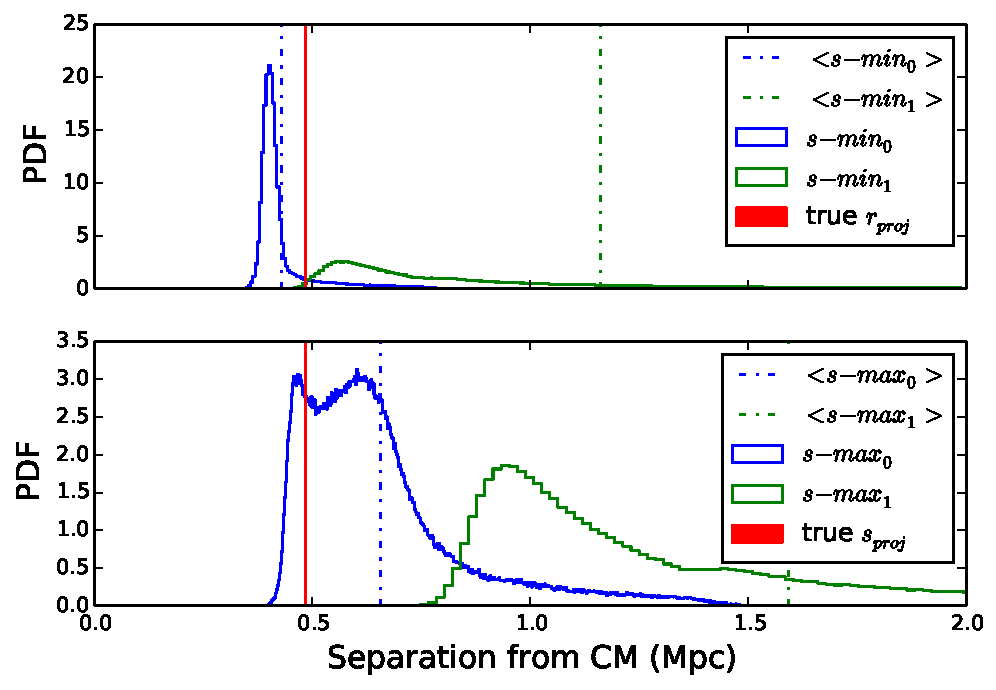
\includegraphics[width=\linewidth]{default_prior_bounds.pdf}
	\caption{Comparison of the observed position of the relic (red) with the
	predicted position from the two simulated merger scenarios (blue for
	outgoing and green for the incoming scenario). The outgoing scenario
	is more favored than the incoming scenario since the shock speed is
	unlikely to travel at much less than $0.6 v_{3D,1}(t_{col}$ for a
	significant period of time. Default priors were
	used for this figure. Alternate version of this figure with the polarization prior applied can
	be found in Appendix \ref{app: results}. \label{fig: positionprior}}
\end{figure}

\begin{figure} 
	\includegraphics[width =\linewidth]{elGordoTSCwithBullet_revC.png}
	\caption{The marginalized outgoing time-since-collision (TSC_0) vs 3D
velocities ($v_{3D}$) of El Gordo and the Bullet Cluster. (to add
descriptions of the different filters used) }
\end{figure}

\begin{figure}
	\includegraphics[width=\linewidth]{TSC_0_vs_v_3d_col_histplot2d_combine2.png}
	\caption{The marginalized output PDF of the outgoing time-since-collision
(TSC$_0$) vs. the 3D velocity at the time of collision for El Gordo. (to
add more description about contours) }
	\label{fig:TSC_v3D}
\end{figure}

%%%%% list of stuff to talk about --- 
% - explain what the figure means 
% - how we intrepret that the outgoing scenario is more likely 
% - why we are leaving all the figures of incoming scenario in the appendix
%   / upon request   
% 
%Bse on the time evolution of radio relic, we speculate that El Gordo has already reached its apoapsis and the two subclusters are heading for another merger.
%%This degeneracy between $TSC_0$ and $TSC_1$ that
%is not resolved by taking the separation constrain from the radio relic. 

%the post-collision estimate of the
%time-since-collision ($TSC_0$), the pre-collision estimate of the
%time-since-collision ($TSC_1$) and the time between collisions ($T$).
%We pick the post-collision time-since-collision estimate ($TSC_0$) of Gyr to be representative of the observed status of El Gordo, instead of the pre-collision time-since-collision estimate ($TSC_1$). While the simulation models both scenarios either the subclusters are approaching each other (incoming) or they have already passed through each
%other and are moving apart (outgoing), the presence of the radio relic rules out the possibility that the two subclusters still have not encountered each other. 
%However, this does not exclude the possibility of having the subcluster
%approaching each other again after reaching apoapsis.  
%%\citet{b9} have reported that the simultaneous optical and near-IR data of
%%AC Her can be fitted by a combination of two blackbodies at 5680 and
%1800\,K, representing, respectively, the stellar and

